
\documentclass[smaller,aspectratio=169, toc=bibliography]{beamer}
\usepackage[language=en,color=fb3, footlinescaling=0.90]{UK-beamer}
\usepackage{graphicx}
\usepackage{amsmath, amsthm, amssymb}
\usepackage{amsfonts}
\usepackage{xspace}
\usepackage{color}
\usepackage{subfigure}
\usepackage{float}
%\usepackage{svg}
%\usepackage{url}
\usepackage{tikz}
\usepackage{pgfplots}
%\pgfplotsset{compat=1.18}
\usepackage[T1]{fontenc}
\pgfplotsset{compat=1.17}
%%%%%%%%%%%%%%%%%

\setbeamertemplate{blocks}[framed]
%\setbeamertemplate{caption}[default]
%\setbeamersize{description width=15mm}

\setbeamertemplate{footline}[classic]
\setbeamertemplate{background canvas}[logotopright]
%%%%%%%%%%%%%%%%%




\begin{document}


\title[Modeling infectious diseases in mixed household structures]{Modeling infectious diseases in mixed \\ household structures}
%\subtitle{Master Thesis \\ Mathematical Modeling Of Complex Systems}
\author{Shrawan Parajuli}
%\institute{Mathematical Institute\\University of Koblenz}
\institute{Mathematisches Institut\\Universität Koblenz}
\date{11/01/2024}



\begin{frame}

\titlepage
\end{frame}


\begin{frame}{\contentsname}
\tableofcontents
\end{frame}

\section{Background Study}
\begin{frame}[fragile]{Background Study}
\begin{itemize}
\item Emergence of infectious diseases is concerning. 
\item spread of infectious disease gradually decreases due to immunity or become endemic due to lack of healthcare facilities. 
\item Study of infectious disease is an interdisciplinary fields is studied with different perspectives and purposes.
%Approach to understand the spread of infection is with different purposes from data to find analytical solution and qualitative behaviour of solution. 
\item Considering household structure has been an useful way of understanding spread of infectious diseases(for eg. Influenza) and it can be done with different epidemiological models such as  SIS (Susceptible-Infectious-Susceptible). 
\item Also, the dynamics of infectious diseases is considered by studying equilibria. 
\end{itemize}
\tiny{Reference- [1],[3]}
\end{frame}

\section{Objectives}
\begin{frame}[fragile]{Objectives}
\begin{itemize}
\item To analyze equilibria (Disease-Free Equilibrium(DFE) and Endemic Equilibrium(EE)).  
\item To observe the influence of infection and recovery parameters in Population dynamics. 
% such as between-household infection rate($\alpha$), within-household infection rate($\beta$) and recovery parameters($\gamma$)
\end{itemize}
\end{frame}

\section{Model and Method}
\begin{frame}[fragile]{Model and Method}
\begin{itemize}

\item Single Household (SHH) using SIS model.  

%the rate of infection from outside the household is proportional to the fraction for the population that is infectious.
\item Master equation describes the time-evolution of $P_k$, $P_k$ denotes the probability having k infected individuals and (N-k) denotes susceptible in a given household size N,
\item External infection rate, $\epsilon=\tilde{\alpha}\frac{I}{T_p}$, 
\item Homogeneous household, Expectation: $\mathbb{E}I_H=\sum_{k=0}^N k*P_k$.
\item $\frac{I}{T_p} \approx \frac{M_H*\mathbb{E}I_H}{M_H*N}=\frac{\mathbb{E}I_H}{N}=\frac{1}{N}{\sum_{k=0}^N kP_k}$
\item In the SHH-N Model we have $$\epsilon=\frac{\alpha}{N}{\mathbb{E}I_H}=\frac{\alpha}{N}{\sum_{k=0}^N kP_k}$$
% with a suitable parameter $\alpha$.
\end{itemize}
\tiny{Reference- [1]}
\end{frame}

\subsection*{Model and Method: State transition}
\begin{frame}[fragile]{Model and Method: State transition}

\begin{itemize}
	\item State transition in (SHH)
\begin{figure}[H]
\centering
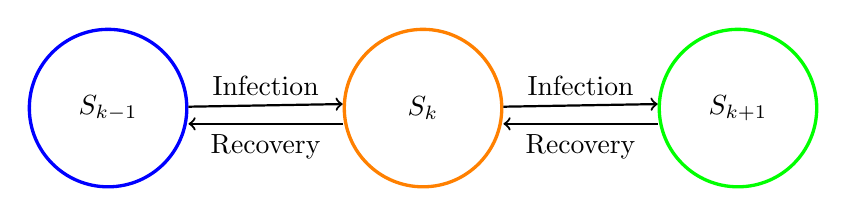
\begin{tikzpicture}[node distance=4cm, auto]
    % Define nodes
    \node [draw=orange, very thick, circle, minimum size=2cm] (Si) {$S_k$};
    \node [draw=blue, very thick, circle, minimum size=2cm, left of=Si] (Siminus) {$S_{k-1}$};
    \node [draw=green, very thick, circle, minimum size=2cm, right of=Si] (Siplus) {$S_{k+1}$};
    
    % Arrows from Sk-1 to Si and from Sk to Sk-1
    \draw[->, thick] ([yshift=0.2cm]Siminus) -- node[above]{Infection} ([yshift=0.2cm]Si);
    
    \draw[->, thick] ([yshift=-0.2cm]Si.west) -- node[below]{Recovery} ([yshift=-0.2cm]Siminus.east);
    
    % Arrows from Sk to Sk+1 and from Sk+1 to Sk
    \draw[->, thick] ([yshift=0.2cm]Si) -- node[above]{Infection} ([yshift=0.2cm]Siplus);
    
    \draw[->, thick] ([yshift=-0.2cm]Siplus.west) -- node[below]{Recovery} ([yshift=-0.2cm]Si.east);
\end{tikzpicture}
\caption{SHH diagram for state transition}
\label{SHH state transition diagram}
\end{figure}
\end{itemize}
\end{frame}

\subsection*{Model and Method: SHH-N}
\begin{frame}[fragile]{Model and Method: SHH-N}
\begin{columns}[c]
\column{0.5\textwidth}
        \begin{center}
        \includegraphics[width=\linewidth]{screenshot/general_SHHN.png}
        \caption{SHH-N} 
        \end{center}
        \column{0.5\textwidth}
        \begin{center}
        \begin{itemize}
        		\item Positive Contribution
		\begin{itemize}
				\item (external infection) $S_{k-1}\rightarrow S_{k}$ , $k \in \{1,2,..N\}$, 
				\item (internal infection) $S_{k-1}\rightarrow S_{k}$ , $k \in \{2,..N\}$
				\item (recovery) $S_{k+1}\rightarrow S_{k}$ , $k \in \{0,..N-1\}$,
		\end{itemize}  

			\item Negative Contribution
		\begin{itemize}
			\item (external infection) $S_{k}\rightarrow S_{k+1}$ , $k \in \{0,..N-1\}$, 
			\item (internal infection) $S_{k}\rightarrow S_{k+1}$ , $k \in \{1,..N-1\}$
			\item (recovery) $S_{k}\rightarrow S_{k-1}$ , $k \in \{1,..N\}$, 
		\end{itemize}
        		\end{itemize} 
        	\end{center}
	\end{columns}
\end{frame}


%\begin{frame}{master equation}

%\begin{itemize}
%\item The general form of the  master equations can be written as:
%\begin{equation}
%	\label{general_discrete_master_equation} 
%\frac{dP_k}{dt} =T_{(k-1)k}P_{k-1}-T_{k(k-1)}P_k+T_{(k+1)k}P_{k+1}-T_{k(k+1)}P_k 
%\end{equation} 

%\end{itemize}

%\end{frame}

\subsection*{Model and Method : SHH-N = 1,2}
\begin{frame}[fragile]{Model and Method : SHH-N = 1,2}	
\begin{itemize}	
	\item General Master Equation for SHH in case of household size N=1,(SIS Model)
		%Setting N:=1 in equation \eqref{masterSHH} we get:

%\subsubsection*{$\frac{dP_0}{dt}$ for SHH in case N=1}
	\begin{equation*}
		\begin{aligned}
			{\frac{dP_0}{dt}} & = \gamma P_{1} - \alpha P_{1} P_{0} \\					
		\end{aligned}
	\end{equation*}

%\subsubsection*{$\frac{dP_1}{dt}$ for SHH in case N=1}

	\begin{equation*}
		\begin{aligned}
			{\frac{dP_1}{dt}} & = \alpha P_{1} P_{0} - \gamma P_{1} \\
		\end{aligned}
	\end{equation*}
	\item General Master Equation for SHH in case of household size N=2,
%	\subsubsection*{$\frac{dP_0}{dt}$ for SHH in case N=2}
\begin{equation*}
	\begin{aligned}
		{\frac{dP_0}{dt}} & = \gamma P_{1} - 2 (\frac{\alpha}{2}P_{1} + \alpha P_{2}) P_{0}					
	\end{aligned}
\end{equation*}
%\subsubsection*{$\frac{dP_1}{dt}$ for SHH in case N=2}
\begin{equation*}
	\begin{aligned}
		{\frac{dP_1}{dt}} & =2 (\frac{\alpha}{2}P_{1} + \alpha P_{2}) P_{0} + 2 \gamma P_{2} - (\frac{\alpha}{2}P_{1} + \alpha P_{2}) P_{1} - \beta P_{1} - \gamma P_{1}
	\end{aligned}
\end{equation*}
%\subsubsection*{$\frac{dP_2}{dt}$ for SHH in case N=2}
\begin{equation*}
	\begin{aligned}
		{\frac{dP_2}{dt}} & = (\frac{\alpha}{2}P_{1} + \alpha P_{2}) P_{1} + \beta  P_{1} - 2 \gamma P_{2}
	\end{aligned}
\end{equation*} 

\end{itemize}
\tiny{Reference- [1]}
\end{frame}

\subsection*{Model and Method : Analytical Approach }
\begin{frame}[fragile]{Model and Method : Analytical Approach }
\begin{itemize}
\item Non-linear differential equations is studied with stability analysis, phase portraits and Numerical simulation.  
\item Total infection rate :
$$ \frac{d\mathbb{E}[I_H]}{dt} = \frac{dP_1}{dt} + 2\frac{dP_2}{dt} $$\\  
\begin{equation*}
\label{Total Infection rate}
   I_{Total} =  \int_{0}^{T} \mathbb{E}[I_H(t)] \,dt  
\end{equation*}
%\item Total recovered rate: 
%\begin{equation*}
%\label{Total Recovered rate}
%R_{Total} =  \gamma I_{Total} 
%\end{equation*}	

\item Equilibrium 

\begin{itemize}
	\item DFE, $\displaystyle lim_{t\rightarrow\infty}(P_0(t),P_1(t),P_2(t)) = (1, 0, 0)$ . 
	\item In EE, $\displaystyle lim_{t\rightarrow\infty} (P_0(t),P_1(t),P_2(t)) \neq (1,0,0)$ (or (1,0,0) does not exist ).
\end{itemize}
%where t represents time.\\


\item In equilibrium :   
\begin{equation*}
\label{function_pk}
	\begin{aligned}
	   	dP_k/dt = f_k(P_k) = 0   
	\end{aligned}	 
\end{equation*}

\end{itemize}
\end{frame}

%\section{Model and Method : 2i}
%\begin{frame}[fragile]{Model and Method : 2i}
%\begin{itemize}
%The jacobian matrix($\emph{J}$) is ,\\ 
%$\begin{bmatrix}
%\label{Model and method jacobian}
%\frac{\partial f_0}{\partial P_0}(P_{0}^*,P_{1}^*,P_{2}^*) & \frac{\partial f_0}%{\partial P_1}(P_{0}^*,P_{1}^*,P_{2}^*) & \frac{\partial f_0}{\partial P_2}(P_{0}^*,P_{1}^*,P_{2}^*) \\
%\\
%\frac{\partial f_1}{\partial P_0}(P_{0}^*,P_{1}^*,P_{2}^*) & \frac{\partial f_1}{\partial P_1}(P_{0}^*,P_{1}^*,P_{2}^*) & \frac{\partial f_1}{\partial P_2}(P_{0}^*,P_{1}^*,P_{2}^*) \\
%\\
%\frac{\partial f_2}{\partial P_0}(P_{0}^*,P_{1}^*,P_{2}^*) & \frac{\partial f_2}{\partial P_1}(P_{0}^*,P_{1}^*,P_{2}^*) & \frac{\partial f_2}{\partial P_2}(P_{0}^*,P_{1}^*,P_{2}^*) \\
%\\
%\end{bmatrix}$
%\end{itemize}
%\end{frame}

\subsection*{Model and Method : Linearization, DFE}
\begin{frame}[fragile]{Model and Method : Linearization, DFE}
\begin{itemize}
\item Linearization in SHH-2
\item DFE, Jacobian Matrix ($\emph{J}$) at $(1, 0, 0)$
\begin{equation*}
\label{jacobian at equilibrium point}
\begin{aligned}
		\left(\begin{array}{rrr}
		0 & -\alpha + \gamma & -2 \, \alpha \\
		0 & \alpha - \beta - \gamma & 2 \, \alpha + 2 \, \gamma \\
		0 & \beta & -2 \, \gamma
		\end{array}\right)
\end{aligned}
\end{equation*}

\item characteristic equation of the form is \( | \emph{J} - \lambda E | \) = 0,

\begin{equation*}
\label{submatrix}
\begin{aligned}
	\left(\begin{array}{rr}
		\alpha - \beta - \gamma & 2 \, \alpha + 2 \, \gamma \\
		\beta & -2 \, \gamma
		\end{array}\right)
\end{aligned}
\end{equation*}

\begin{equation*}
\label{eigenvalue} 
\begin{aligned}
&\lambda_{i} = \frac{Tr - \sqrt{Tr^2-4D}}{2}\\
&\lambda_{ii} = \frac{Tr + \sqrt{Tr^2-4D}}{2}    
\end{aligned}
\end{equation*}
\end{itemize}
\tiny{Reference- [2]}
\end{frame}

\subsection*{Model and Method : Trace and Determinant}
\begin{frame}[fragile]{Model and Method : Trace and Determinant}
\begin{itemize}

\item Let A be 2 X 2 square matrix of form written in  
\begin{equation*}
\label{generalsubmatrix}
\begin{aligned}
	\left(\begin{array}{rr}
		a_{11} & a_{12} \\
		a_{21} & a_{22}
		\end{array}\right)
\end{aligned}
\end{equation*}
\item $Trace(Tr) = a_{11} + a_{22} = \alpha - \beta - 3\gamma $
\\
\item $Determinant(D) = a_{11}a_{22} - a_{12}a_{21} = 2(\gamma^2 - \alpha(\beta + \gamma)) $ 
%\paragraph*{Trace(Tr) and Determinant(D)}:\\
%We compare \ref{submatrix} with \ref{generalsubmatrix} and write $Tr$ as 
%\begin{equation}
%\label{Trace} 
%\begin{aligned}
%&Tr = \alpha - \beta - 3\gamma 
%\end{aligned}
%\end{equation}

%And also we compare \ref{submatrix} with \ref{generalsubmatrix} and  write $D$ as 
%\begin{equation}
%\label{Determinant}
%\begin{aligned}
%&D = 2(\gamma^2 - \alpha(\beta + \gamma))
%\end{aligned}
%\end{equation}

\end{itemize}
\end{frame}

\subsection*{Model and Method : Endemic Equilibrium}
\begin{frame}[fragile]{Model and Method : EE }
\begin{itemize}
\item EE, endemic equilibrium point $(P_0, P_1, P_2)$ or $(P_0, P_1, 1 - P_0 - P_1 )$  

\item $P_1$, 
\begin{equation}
\label{positive root of P1}
	\begin{aligned}
	&P_1 = \frac{2\alpha P_0(1 - P_0)}{(\gamma + \alpha P_0 )}
	\end{aligned}
\end{equation}
\item positive root $P_0$,
\begin{equation}
\label{positive root of P0}
	\begin{aligned}
		&P_0 = \frac{\gamma}{2\alpha\beta}(-( \alpha + \beta ) + \sqrt{( \alpha + \beta )^2 + 4\beta\gamma})
	\end{aligned}
\end{equation}
\item jacobian at ($P_0$,$P_1$,1-$P_0$-$P_1$)
\begin{equation}
\label{jacobian at endemic equilibrium point}
\begin{aligned}
		\left(\begin{array}{rrr}
		-\alpha(2 - 2P_0 - P_1) & -\alpha P_0 + \gamma & -2 \, \alpha P_0 \\
		\alpha(2 - 2P_0 - P_1)  & P_0(1 + \alpha) -1 - \beta - \gamma & 2 \, \alpha P_0 - \alpha P_1  + 2 \, \gamma \\
		0 & \alpha(1 - P_0 ) + \beta & \alpha P_1 -2 \, \gamma
		\end{array}\right)
\end{aligned}
\end{equation}
\end{itemize}
\end{frame}

\section{Simulation and Results}
\begin{frame}[fragile]{Simulation and Results}
\begin{itemize}
\item Numerical method: Runge-Kutta Method, $(RK45)$ 
\item Initial conditions, $P_0$ is $P_0(0)= 0.98$ , $P_1$ is $P_1(0)=0.02$  and  $P_2$ is $P_2(0)=0$,
\item timestep : [0,50]
\item parameters
\begin{itemize}
	\item $\alpha$ : between-household infection rate. 
	\item $\beta$ : within-household infection rate. 
	\item $\gamma$ : household recovery rate
\end{itemize} 
\item vary only one parameter and keep the other two parameter fixed 
\item regular spaced (0.2,0.3,0.4,0.5,0.6,0.7,0.8) rates
\item initial rates , $\alpha$ = 0.4, $\beta$ = 0.2, $\gamma$ = 0.2 
\item for example : Influenza recovered rate 0.2 ( takes 5 days to recover )
\end{itemize}
\end{frame}

%
% try 
%

\subsection*{Simulation and Results:($\alpha$) }
\begin{frame}{Probability of household state vs time ($\alpha$)}

%alpha
\begin{columns}[c]
        \column{0.6\textwidth}
        \begin{center}
        \includegraphics[scale=0.3]{screenshot/7alphaP_kvstime.png}
        \end{center}
		
\end{columns}
\end{frame}

\subsection*{Simulation and Results:($\alpha$): cont. }
\begin{frame}{Probability of household state vs time ($\alpha$):cont.}

%alpha
\begin{columns}[c]
        \column{0.5\textwidth}
        \begin{center}
        \begin{itemize} 
        \label{time step of steady values of probability}
        \item Probability of household states($P_k$)		
		\begin{equation*}
 				|P_{k_{t_{i+1}}}-P_{k_{t_{i}}}| < 10^{-3}
		\end{equation}
		\item Total infection rate($I_{Total}$) 
		\begin{equation*}
		\label{time step of steady values of total infection}
 				|I_{Total_{t_{i+1}}}-I_{Total_{{t_{i}}}}| < 10^{-3}
		\end{equation}
		\end{itemize}
        \includegraphics[width=\linewidth]{screenshot/10alphaRK_PK.png}
        \includegraphics[width=\linewidth]{screenshot/4alphaTITRTT.png}
        \end{center}
        \column{0.3\textwidth}
        \begin{center}
        \includegraphics[scale=0.2]{screenshot/1P_kvsAlpha.png}
        \caption{$P_0$,$P_1$,$P_2$ on y-axis and $\alpha$ on x-axis}
        \end{center} 

\end{columns}
\end{frame}

%beta
\subsection*{Simulation and Results:($\beta$) }
\begin{frame}{Probability of household state vs time ($\beta$)}

\begin{columns}[c]
        \column{0.6\textwidth}
        \begin{center}
        \includegraphics[scale=0.3]{screenshot/8betaP_kvstime.png}
        \end{center}		
\end{columns}
\end{frame}

\subsection*{Simulation and Results:($\beta$): contd. }

\begin{frame}{Probability of household state vs time ($\beta$):cont.}
\begin{columns}[c]
        \column{0.5\textwidth}
         \begin{center}
        \begin{itemize} 
        \label{time step of steady values of probability}
        \item Probability of household states($P_k$)		
		\begin{equation*}
 				|P_{k_{t_{i+1}}}-P_{k_{t_{i}}}| < 10^{-3}
		\end{equation}
		\item Total infection rate($I_{Total}$) 
		\begin{equation*}
		\label{time step of steady values of total infection}
 				|I_{Total_{t_{i+1}}}-I_{Total_{{t_{i}}}}| < 10^{-3}
		\end{equation}
		\end{itemize}
        \includegraphics[width=\linewidth]{screenshot/11betaRK_PK.png}
        \includegraphics[width=\linewidth]{screenshot/5betaTITRTT.png}  
        \end{center}
        \column{0.3\textwidth}
        \begin{center}
        \includegraphics[scale=0.2]{screenshot/2P_kvsbeta.png}
        \caption{$P_0$,$P_1$,$P_2$ on y-axis and $\beta$ on x-axis}
        \end{center}  
\end{columns}
\end{frame}


\subsection*{Simulation and Results:($\gamma$) }

%gamma 
\begin{frame}{Probability of household state vs time ($\gamma$)}
\begin{columns}[c]
        \column{0.6\textwidth}
        \begin{center}
        \includegraphics[scale=0.3]{screenshot/9gammaP_kvstime.png}
        \end{center}
\end{columns}
\end{frame}

\subsection*{Simulation and Results:($\gamma$): contd. }

%gamma 
\begin{frame}{Probability of household state vs time ($\gamma$):cont.}
\begin{columns}[c]
        \column{0.5\textwidth}
                \begin{center}
        \begin{itemize} 
        \label{time step of steady values of probability}
        \item Probability of household states($P_k$)		
		\begin{equation*}
 				|P_{k_{t_{i+1}}}-P_{k_{t_{i}}}| < 10^{-3}
		\end{equation}
		\item Total infection rate($I_{Total}$) 
		\begin{equation*}
		\label{time step of steady values of total infection}
 				|I_{Total_{t_{i+1}}}-I_{Total_{{t_{i}}}}| < 10^{-3}
		\end{equation}
		\end{itemize}
        \includegraphics[width=\linewidth]{screenshot/12gammaRK_PK.png}
        \includegraphics[width=\linewidth]{screenshot/6gammaTITRTT.png}
        \end{center}
        \column{0.3\textwidth}
        \begin{center}
        \includegraphics[scale=0.2]{screenshot/3P_kvsgamma.png}
        \caption{$P_0$,$P_1$,$P_2$ on y-axis and $\gamma$ on x-axis}
       \end{center}
\end{columns}
\end{frame}
%\subsection*{Simulation and Results:($\gamma$): $I_{Total}$,Timestep}
%\begin{frame}{$I_{Total}$,Timestep varying ($\alpha$, $\beta$, $\gamma$)}
%\begin{columns}[c]
%        \column{0.5\textwidth}
%        \begin{center}
%            \includegraphics[width=\linewidth]{screenshot/4alphaTITRTT.png}
%        \caption{varying $\alpha$} 
%        \end{center}
%        \begin{center}
%            \includegraphics[width=\linewidth]{screenshot/5betaTITRTT.png}
%         \caption{varying $\beta$}
%         \end{center}
%         \begin{center}
%             \includegraphics[width=\linewidth]{screenshot/6gammaTITRTT.png}
%         \caption{varying $\gamma$}
%       \end{center}
%        \column{0.5\textwidth}
%        \begin{center}
%        \begin{itemize}
%        \item  varying(gradually increasing) $\alpha$ - > $I_{Total}$ $\uparrow$, %Timestep $\downarrow$
%         %$R_{Total}$ $\uparrow$,Timestep $\downarrow$
%        \item varying $\beta$ - > $I_{Total}$ $\uparrow$ , Timestep $\downarrow$
        %$R_{Total}$ $\uparrow$,Timestep $\downarrow$
%        \item varying $\alpha$ - > $I_{Total}$ $\downarrow$ , Timestep $\uparrow$
        %$R_{Total}$ $\downarrow$,Timestep $\uparrow$
%        \end{itemize}
%        \end{center}
%\end{columns}
%\end{frame}

\section*{Disease-Free equilibrium}
\begin{frame}{Disease-Free equilibrium}
\begin{columns}
\column{0.5\textwidth} % Left column for the figure
\begin{center}
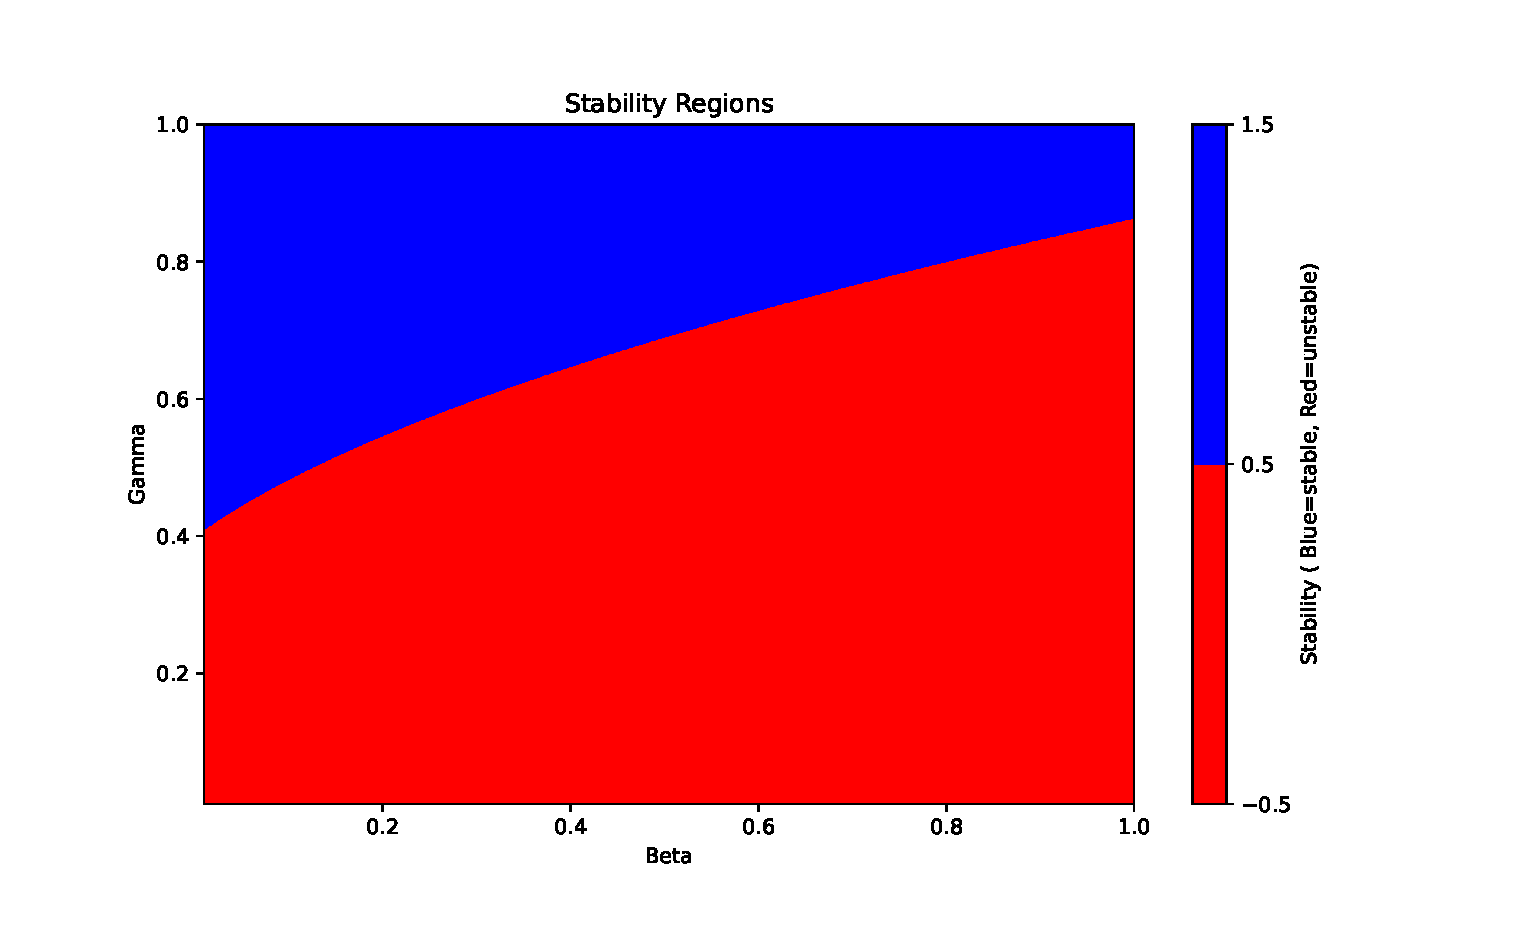
\includegraphics[width=\linewidth]{img/stability.eps}
\caption{$\gamma$ range on $y-axis$ and $\beta$ range on $x-axis$ with constant $\alpha$ at 0.4.}
\label{regions of stability and unstability}
\end{center}
\column{0.5\textwidth} % Right column for key points
\begin{itemize}
\item \textbf{eigenvalues :} $\lambda_{i} < 0$, $\lambda_{ii} < 0$
\item \textbf{case :} $ Tr < 0$ and $Tr > \sqrt{Tr^2-4D} $ , where  $D > 0$ and $Tr^2 > 4D $
\item \textbf{Parameter :} $ Tr < 0 $, means \( \alpha < \beta + 3\gamma \) and $ D > 0 $ means \( \alpha < \frac{\gamma^2}{\beta + \gamma} \)
\end{itemize}
\end{columns}
\end{frame}


\section*{Endemic equilibrium: $\alpha$}
\begin{frame}{Endemic equilibrium: varying $\alpha$}
\begin{columns}[c]
\column{0.4\textwidth}
\begin{center}
%\includegraphics[scale=0.4]{screenshot/10alphaRK_PK.png}
\includegraphics[width=\linewidth]{screenshot/10alphaRK_PK.png}
\caption{Runge-Kutta Method: $\alpha$} 
\end{center}
\begin{center}
%\includegraphics[scale=0.4]{screenshot/13alphaEE_PK.png}
\includegraphics[width=\linewidth]{screenshot/13alphaEE_PK.png}
\caption{Equilibrium: $\alpha$} 
\end{center}
\column{0.5\textwidth} % Right column for key points
\begin{itemize}
\item \textbf{Numerical values: } RK method and endemic equilibrium values are similar.
 
\item \textbf{$P_0$ = } \( \frac{\gamma}{2\alpha\beta}(-( \alpha + \beta ) + \sqrt{( \alpha + \beta )^2 + 4\beta\gamma}) \)
\item \textbf{$P_1$ = } \( \frac{2\alpha P_0(1 - P_0)}{(\gamma + \alpha P_0 )}\) 
\item \textbf{$P_2$ = } $1 - P_0 - P_1$ 
\item value of $P_0$ affects value in $P_1$ and summation of both $P_0$ and $P_1$ results change in $P_2$. 
\item \textbf{linearization : } Two negative eigenvalues(stable). 
\end{itemize}
\end{columns}
\end{frame}

\section*{Endemic equilibrium: $\beta$ }
\begin{frame}{Endemic equilibrium: varying $\beta$}     
\begin{columns}[c]   
        \column{0.4\textwidth}
            \begin{center}
                \includegraphics[width=\linewidth]{screenshot/11betaRK_PK.png}
                \caption{Runge-Kutta Method : $\beta$}
            \end{center} 
              \begin{center}
                \includegraphics[width=\linewidth]{screenshot/14betaEE_PK.png}
                \caption{Equilibrium: $\beta$}
            \end{center} 
            \column{0.5\textwidth} % Right column for key points
            \begin{itemize}
\item \textbf{Numerical values: } RK method and endemic equilibrium values are similar.
  
\item \textbf{$P_0$ = } \( \frac{\gamma}{2\alpha\beta}(-( \alpha + \beta ) + \sqrt{( \alpha + \beta )^2 + 4\beta\gamma}) \)
\item \textbf{$P_1$ = } \( \frac{2\alpha P_0(1 - P_0)}{(\gamma + \alpha P_0 )}\) 
\item \textbf{$P_2$ = } $1 - P_0 - P_1$ 
\item value of $P_0$ affects value in $P_1$ and summation of both $P_0$ and $P_1$ results change in $P_2$.
\item \textbf{linearization : } Two negative eigenvalues(stable). 
            \end{itemize}
\end{columns}
\end{frame}

\section*{Endemic equilibrium: $\gamma$ }

\begin{frame}{Endemic equilibrium: varying $\gamma$}
\begin{columns}[c]
            \column{0.4\textwidth}
            \begin{center}
                \includegraphics[width=\linewidth]{screenshot/12gammaRK_PK.png}
                \caption{Runge-Kutta Method : $\gamma$}
            \end{center}
             \begin{center}
                \includegraphics[width=\linewidth]{screenshot/15gammaEE_PK.png}
                \caption{Equilibrium: $\gamma$}
            \end{center}
            \column{0.5\textwidth}
            \begin{itemize}
            \item \textbf{Numerical values: } RK method and endemic equilibrium values are similar.
\item \textbf{$P_0$ = } \( \frac{\gamma}{2\alpha\beta}(-( \alpha + \beta ) + \sqrt{( \alpha + \beta )^2 + 4\beta\gamma}) \)
\item \textbf{$P_1$ = } \( \frac{2\alpha P_0(1 - P_0)}{(\gamma + \alpha P_0 )}\) 
\item \textbf{$P_2$ = } $1 - P_0 - P_1$ 
\item value of $P_0$ affects value in $P_1$ and summation of both $P_0$ and $P_1$ results change in $P_2$. 
\item \textbf{linearization : } Two negative eigenvalues(stable).
\end{itemize}
\end{columns}
\end{frame}

\section*{Phase Portraits}
\begin{frame}[fragile]{Phase portraits}
\begin{equation}
\label{two dimension}
\begin{aligned}
 f_0(P_0) &= -\alpha( P_1 + 2( 1 - P_0-P_1 )) P_0 + \gamma P_1 \\
 f_1(P_1) &=  \alpha( P_1 + 2( 1 - P_0 - P_1 )) P_0    \\
        &- ((\alpha/2)( P_1 + 2(1 - P_0 - P_1)) + \beta + \gamma ) P_1  \\
        &+ 2 \gamma ( 1 - P_0 - P_1)        
\end{aligned}
\end{equation}
\end{frame}
\subsection*{Phase Portraits: $\alpha$ }
\begin{frame}{vector plot and stream plot: $\alpha$}
\begin{columns}[c]
        \column{0.3\textwidth}
        \begin{center}
        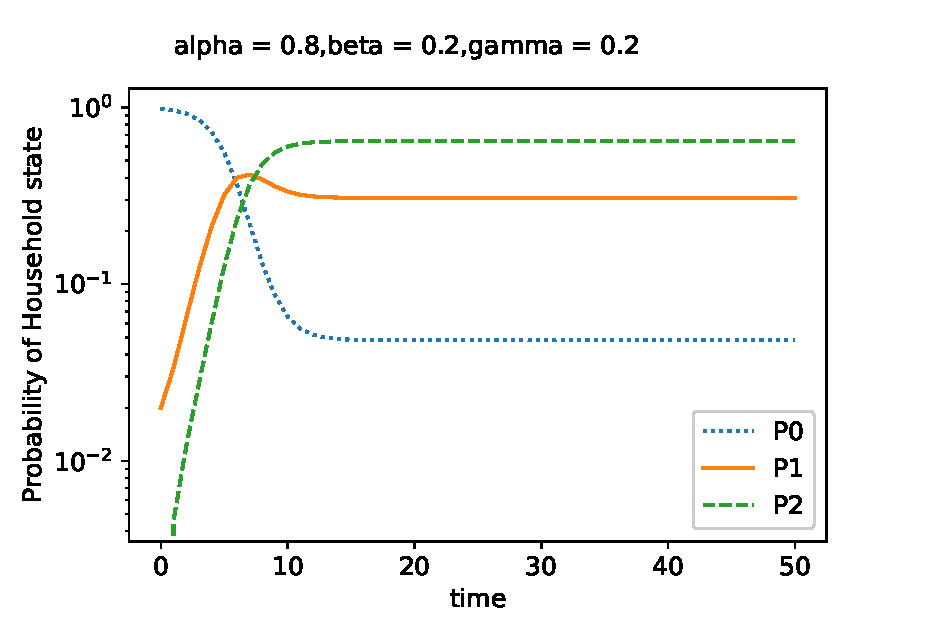
\includegraphics[scale=0.3]{phase_portrait/041_g5.eps}
        \caption{\(\alpha=0.8, \beta=0.2, \gamma=0.2\)} 
        \end{center}
        \column{0.3\textwidth}
        \begin{center}
        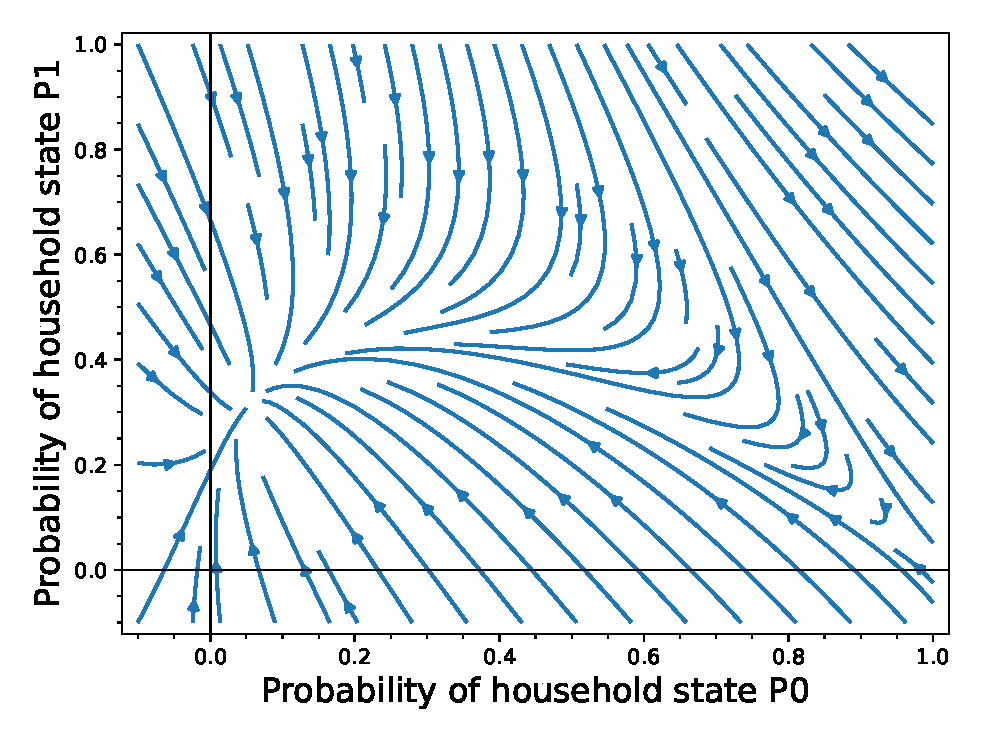
\includegraphics[scale=0.3]{phase_portrait/041_g5s.eps}
        \caption{\(\alpha=0.8, \beta=0.2, \gamma=0.2\)}
        \end{center}  
\end{columns}
\end{frame}

\subsection*{Phase Portraits: $\beta$ }

\begin{frame}{vector plot and stream plot: $\beta$}
\begin{columns}[c]
        \column{0.3\textwidth}
        \begin{center}
        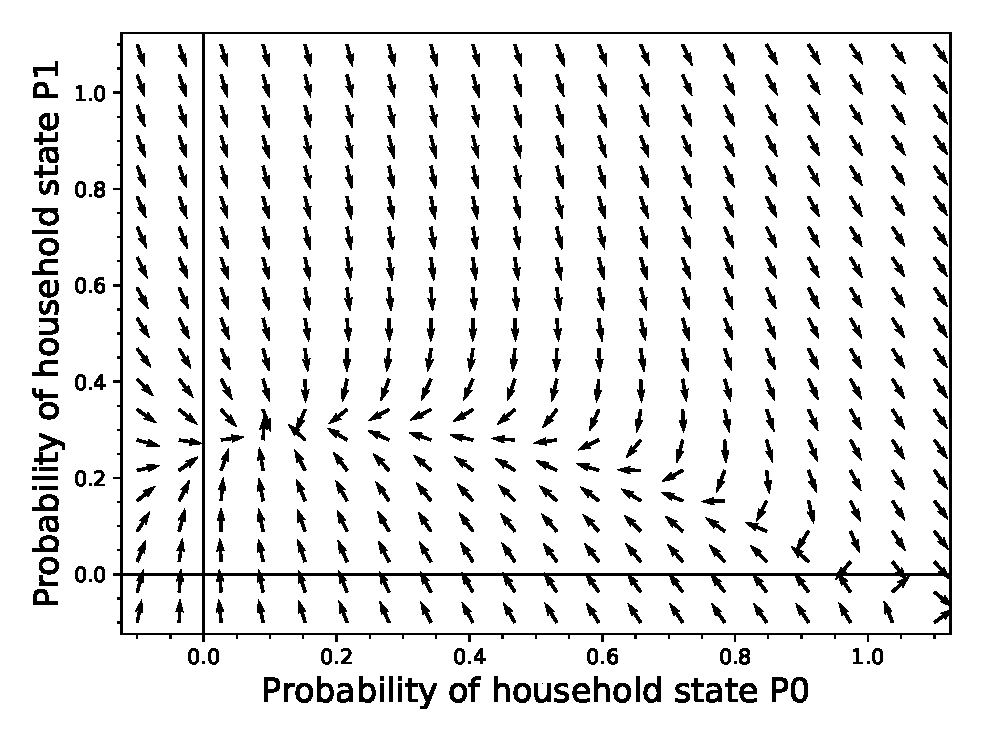
\includegraphics[scale=0.3]{phase_portrait/042_g16.eps}
        \caption{\(\alpha=0.4, \beta=0.5, \gamma=0.2\)} 
        \end{center}
        \column{0.3\textwidth}
        \begin{center}
        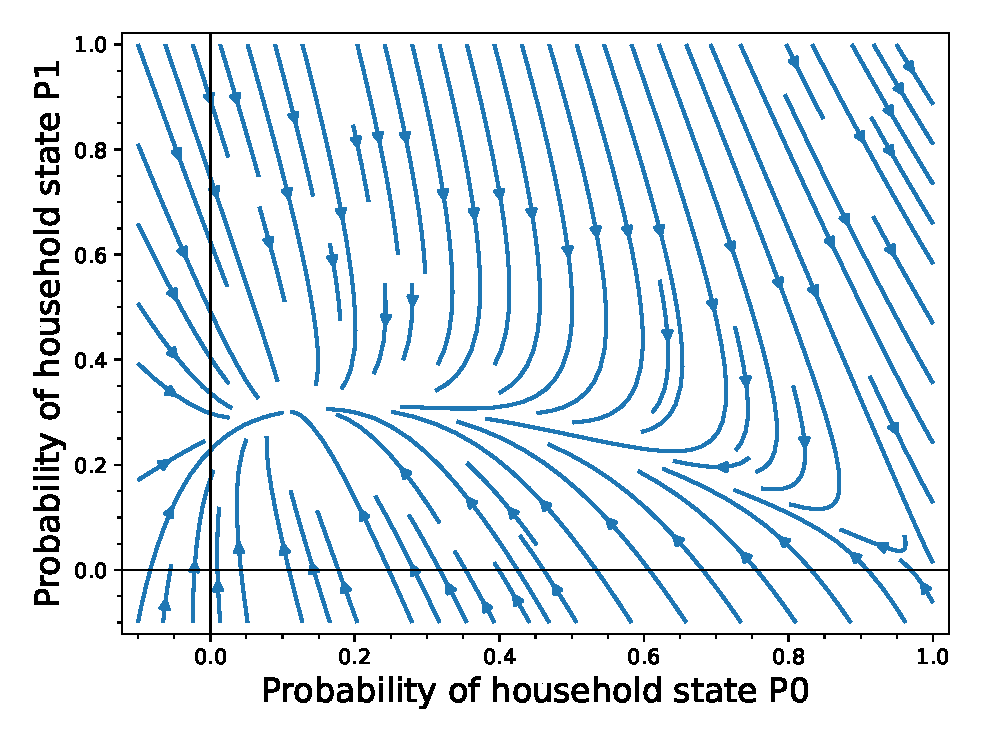
\includegraphics[scale=0.3]{phase_portrait/042_g16s.eps}
        \caption{\(\alpha=0.4, \beta=0.5, \gamma=0.2\)}
        \end{center}  
\end{columns}
\end{frame}


\subsection*{Phase Portraits: $\gamma$ }
\begin{frame}{vector plot and stream plot: $\gamma$}
\begin{columns}[c]
        \column{0.3\textwidth}
        \begin{center}
        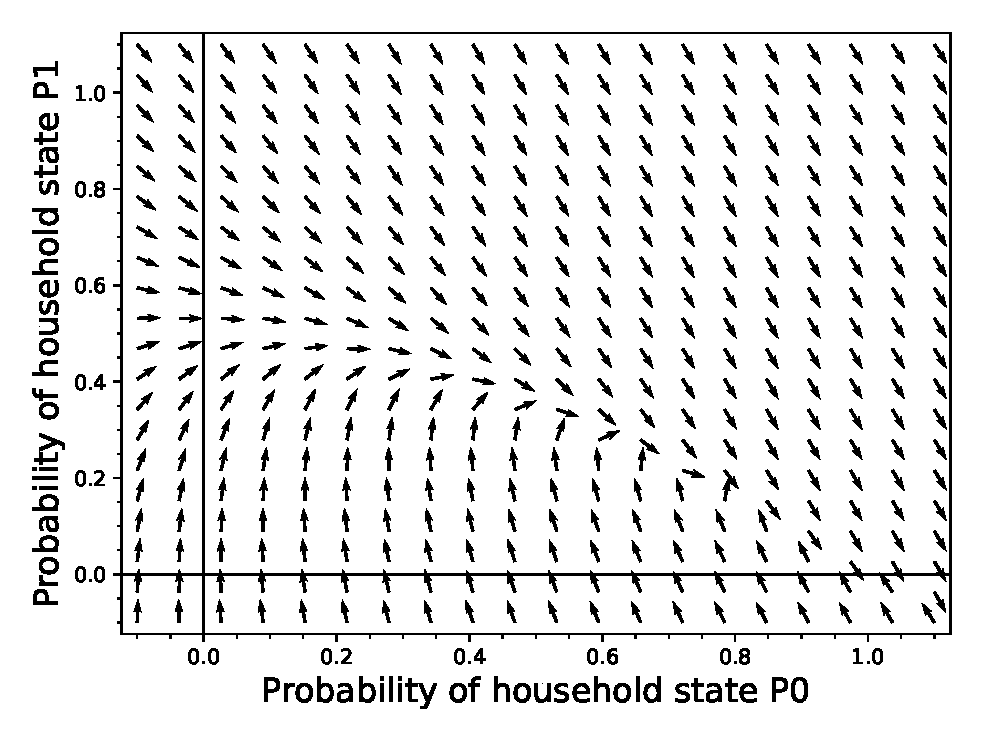
\includegraphics[scale=0.3]{phase_portrait/043_a3.eps}
        \caption{\(\alpha=0.4, \beta=0.2, \gamma=0.6\)} 
        \end{center}
        \column{0.3\textwidth}
        \begin{center}
        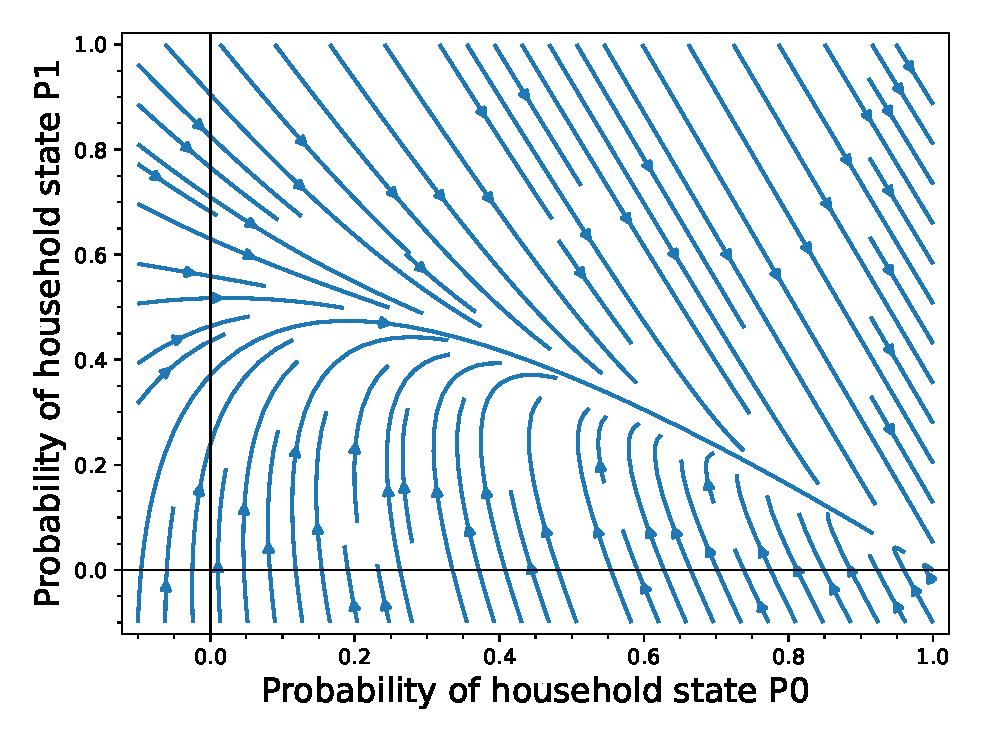
\includegraphics[scale=0.3]{phase_portrait/043_a3s.eps}
        \caption{\(\alpha=0.4, \beta=0.2, \gamma=0.6\)}
        \end{center}  
\end{columns}
\end{frame}

\section{Discussion}
\begin{frame}[fragile]{Numerical simulation results discussion }

\begin{itemize}
\item Total Timestep: 
\begin{itemize}
 \item Gradual \textbf{increase} in $\alpha$ and $\beta$, \textbf{decreases} the \textbf{timestep} to reach steady values. 
%for $P_0$,$P_1$,$P_2$, $I_{Total}$ , $R_{Total}$ 
%for $P_0$,$P_1$,$P_2$,$I_{Total}$ , $R_{Total}$ 
 \item In \textbf{comparison}, there is \textbf{decrease} in the timestep for $\alpha$ but an \textbf{increase} in the total timestep \textbf{$\beta$}.
 \item An \textbf{increase} in $\gamma$ \textbf{increases} timestep. %for $P_0$,$P_1$,$P_2$, $I_{Total}$ , $R_{Total}$ 
\end{itemize}  

\item $P_0$,$P_1$,$P_2$ and $I_{Total}$:
\begin{itemize}
 \item An \textbf{increase} in $\alpha$ and $\beta$ leads to a \textbf{decrease} in $P_0$ and $P_1$ but \textbf{increase} in $P_2$ and $I_{Total}$.
 \item when \textbf{ comparing increase } in $\alpha$ and $\beta$: $P_0$ \textbf{decreases more} in increase in $\alpha$ and \textbf{decreases less} in increase in $\beta$ while $P_1$ \textbf{decreases less} in increase in $\alpha$ and \textbf{decrease more} in $\beta$ whereas $P_2$ remains similar for both  in $\alpha$ and $\beta$.
\item while \textbf{comparing} for $I_{Total}$: increase in $\alpha$ \textbf{increases more} in $I_{Total}$ but \textbf{increases less} in gradual increase in $\beta$. 
\item increase in $\gamma$ \textbf{increases} $P_0$ while ($P_1$,$P_2$, $I_{Total}$) \textbf{decreases}. 
\end{itemize}  
\end{itemize}
\end{frame}

\section*{Discussion}
\begin{frame}[fragile]{Further discussion}
\begin{columns}[c]
\column{0.7\textwidth}
\begin{itemize}
\item Stability in gradual increase in $\alpha$,$\beta$ and $\gamma$(till 0.5), EE. 
\item Stability seen at $\gamma$ = 0.6, at ($P_0$ , $P_1$, $P_2$) = ($P_0$,0,0), DFE.
\item At Phase portraits, 
\begin{itemize}
\item where EE stable (sink), DFE is seen unstable (saddle).
\item where DFE is seen stable (sink), EE is seen unstable (saddle).
\end{itemize}
\end{itemize}
\end{columns}
\end{frame}

\section{Conclusion}		
\begin{frame}[fragile]{Conclusion}
\begin{columns}[c]
\column{0.7\textwidth}
\begin{itemize}

\item In summary, a transition from EE to DFE is observed, at $\gamma$ = 0.6, $\alpha$ = 0.4 and $\beta$ = 0.2.
\item Increase in $\alpha$ and $\beta$ leads to EE and increase in $\gamma$ leads to DFE. 
  
 

\end{itemize}
\end{columns}
\end{frame}

\section*{Limitations and future research}
\begin{frame}{Limitations and future research}
\begin{itemize}
\item Limitation : 
\begin{itemize}
\item Mixed household size rather than same household size. 
\item Larger household size rather than only household of size two. 
\item Strategies or policies. 
\item Household structure (space) and behavioural patterns(movement).  
\end{itemize}
\item Further research : 
\begin{itemize}
\item Epidemiological models. 
\item Higher dimension. 
\item Larger population. 
\item lower rates in parameters. 
\item Intervention strategies.
\end{itemize}
\end{itemize}
\end{frame}


\begin{frame}
\frametitle{References}

\scriptsize{[1] Alex Holmes, Mike Tildesley, and Louise Dyson. Approximating steady state distri-
butions for household structured epidemic models. Journal of Theoretical Biology,
534:110974, 2022}\\
~\\

\scriptsize{[2] Carl P. Simon and John A. Jacquez. Reproduction numbers and the stability of
equilibria of si models for heterogeneous populations. SIAM Journal on Applied
Mathematics, 52(2):541{576, 1992}}\\
~\\

\scriptsize{[3] Fred Brauer. Mathematical epidemiology: Past, present, and future. Infectious
Disease Modelling, 2(2):113{127, 2017}} \\
%~\\

%\scriptsize{[4] Robert Morgan. Linearization and stability analysis of nonlinear problems. RoseHulman Undergraduate Mathematics Journal, 16(2):5, 2015}\\
\end{frame}

\begin{frame}
\begin{center}
\textsc{\sffamily{\Large{Thank You}}}\\
\end{center}
\end{frame}

\end{document}